\documentclass[11pt]{article}
\usepackage{fullpage, amsmath, graphicx, epstopdf, tikz, enumitem}
\usepackage[linesnumbered,ruled,vlined]{algorithm2e}
\usetikzlibrary{arrows}
\usepackage{amsthm}
\usepackage{todonotes}
\renewcommand{\baselinestretch}{1.02}
\newcommand{\Q}[1]{\medskip\item {[{\em #1 marks\/}]}\ }
\usepackage{xcolor}
\newif\ifsol
\soltrue
\newcommand{\solution}[1]{{\ifsol \color{red} {#1} \fi}}

\newtheorem{claim}{Claim}

\newcommand{\down}[1]{\left\lfloor #1\right\rfloor}
\newcommand{\up}[1]{\left\lceil #1\right\rceil}

\begin{document}

\hfill CS 341, Spring 2020\par
\hfill Semih Salihoglu

\bigskip
\begin{center}\large\bf Assignment 5 (due Wed, July 22nd, midnight EST)
\end{center}

\noindent{\bf Instructions:}
\begin{itemize}
\item Hand in your assignment using Crowdmark. Detailed instructions are on the course website.
\item Give complete legible solutions to all questions.
\item Your answers will be marked for clarity as well as correctness.
\item For any algorithm you present, you should justify its correctness
(if it is not obvious) and analyze the complexity.
\end{itemize}

\begin{enumerate}

\Q{15}  Let $G = (V,E)$ be a weighted, directed acyclic graph (DAG) with $n$ vertices and $m$ edges, where $m \ge n$. Let $s,t \in V$. We say that a path $v_1,v_2,...,v_l$ is monotone if $w(v_1,v_2) \le w(v_2,v_3) \le \ldots \le w(v_{l-1},v_l)$. We want to compute a shortest monotone path from $s$ to $t$, i.e., a monotone path of the smallest total weight. Give an $O(mn)$-time algorithm using dynamic programming. Your algorithm should return the optimal path in addition to the optimal value. If no such path exists, you can just return ``no". 

\begin{algorithm} [h]
	\caption{ShortestMonotonePath($G(V, E), s, t, W$)}
	$P[n, n - 1]$\\
	$P[s, 0] = (0, - \infty)$\\
	$P[v \neq s, 0] = (\infty, - \infty)$\\
	$path = \{ t \}$\\
	\For{$i = 1, \dots, n - 1$}{
		\For{$v \in V$}{
			$P[v, i] = P[v, i - 1]$
			\For{$u \in inNbr(v)$}{
				\If{$P[u, i - 1].second \leq w(u, v)$}{
					$P[v, i].first = min(P[v, i].first, P[u, i - 1].first + w(u, v))$\\
					$P[v, i].second = w(u, v)$\\
					$path = path \cap \{u\}$\\
				}
			}
		}
	}
	\uIf{$P[t][n - 1].thrid = \emptyset$}{
		\Return{NO}
	}
	\Return{$(path, YES)$}
\end{algorithm}

\textbf{Proof of Correctness:} Since $G$ is a DAG, it does not have negative weight cycles. So we can apply 
Bellman Ford DP algorithm to find a shortest path from $s$ to $t$.\\
Same as BF algorithm, For a path from $s$ to a vertex $v$ with length $i$, the shortest monotone path 
$p_{(v, i)}$ is the minimum value between $p_{(v, i - 1)}$ and $p_{(u, i - 1) + w(u, v)}$ for some $v$'s 
in-neighbour $u$ and $w(u, v)$ is greater than or equal to the weight of the edge that is incident to $u$. 
Meanwhile, the path form $s$ to $u$ is also monotone and the shortest.

\textbf{Runtime Analysis:} For each $i$, the runtime of computing each entry is $|in_neighbour(v)|$. Since we 
check all the vertices of $G$, the inner loop takes $O(m)$ times. Hence $T(n) = O(m n)$.
\newpage
\Q{12}

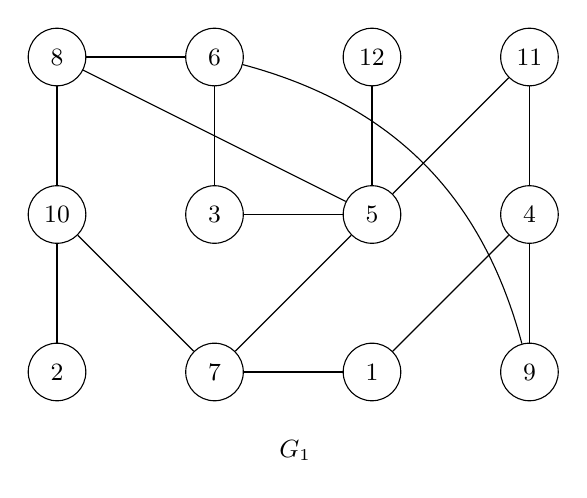
\begin{tikzpicture}
\tikzset{text width={width("10")},
	align=center,
	font=\small}
\tikzset{vertex/.style = {shape=circle,draw,minimum size=1.5em}}
\tikzset{edge/.style = {-,> = latex'}}
% vertices
\node[vertex] (a) at  (0,0) {2};
\node[vertex] (b) at  (2,0) {7};
\node[vertex] (c) at  (4,0) {1};
\node[vertex] (d) at  (6,0) {9};
\node[vertex] (e) at  (0,2) {10};
\node[vertex] (f) at  (2,2) {3};
\node[vertex] (g) at  (4,2) {5};
\node[vertex] (h) at  (6,2) {4};
\node[vertex] (i) at  (0,4) {8};
\node[vertex] (j) at  (2,4) {6};
\node[vertex] (k) at  (4,4) {12};
\node[vertex] (l) at  (6,4) {11};

\node (n) at  (3,-1) {$G_1$};

%edges
\draw[edge] (j) to (i);
\draw[edge] (j) to (f);
\draw[edge] (e) to (a);
\draw[edge] (i) to (e);

\draw[edge] (e) to (b);
\draw[edge] (c) to (b);
\draw[edge] (c) to (h);
\draw[edge] (h) to (d);

\draw[edge] (g) to (f);
\draw[edge] (g) to (k);
\draw[edge] (g) to (l);
\draw[edge] (i) to (g);
\draw[edge][bend left] (j) to (d);
\draw[edge] (l) to (h);
\draw[edge] (b) to (g);
\end{tikzpicture}
\hfill
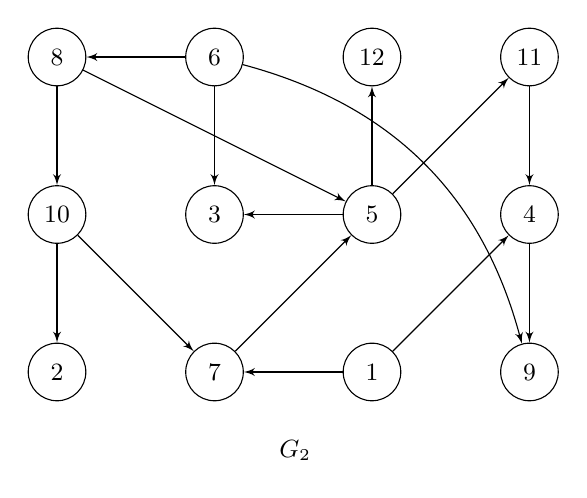
\begin{tikzpicture}
\tikzset{text width={width("10")},
		align=center,
		font=\small}
\tikzset{vertex/.style = {shape=circle,draw,minimum size=1.5em}}
\tikzset{edge/.style = {->,> = latex'}}
% vertices
\node[vertex] (a) at  (0,0) {2};
\node[vertex] (b) at  (2,0) {7};
\node[vertex] (c) at  (4,0) {1};
\node[vertex] (d) at  (6,0) {9};
\node[vertex] (e) at  (0,2) {10};
\node[vertex] (f) at  (2,2) {3};
\node[vertex] (g) at  (4,2) {5};
\node[vertex] (h) at  (6,2) {4};
\node[vertex] (i) at  (0,4) {8};
\node[vertex] (j) at  (2,4) {6};
\node[vertex] (k) at  (4,4) {12};
\node[vertex] (l) at  (6,4) {11};

\node (n) at  (3,-1) {$G_2$};

%edges
\draw[edge] (j) to (i);
\draw[edge] (j) to (f);
\draw[edge] (e) to (a);
\draw[edge] (i) to (e);

\draw[edge] (e) to (b);
\draw[edge] (c) to (b);
\draw[edge] (c) to (h);
\draw[edge] (h) to (d);

\draw[edge] (g) to (f);
\draw[edge] (g) to (k);
\draw[edge] (g) to (l);
\draw[edge] (i) to (g);
\draw[edge][bend left] (j) to (d);
\draw[edge] (l) to (h);
\draw[edge] (b) to (g);
\end{tikzpicture}

\begin{enumerate}
	\Q{2} Run the breadth-first search on the undirected graph $G_1$, starting from vertex 1, and show its final output. When you have to choose which vertex to process next (and that choice is not otherwise specified by the BFS algorithm), use the one with the smallest label. Show the BFS tree by indicating tree edges with solid lines and non-tree edges with dashed lines, and also trace the algorithm (i.e., indicate the action that is taken at every time step).
	\begin{center}
	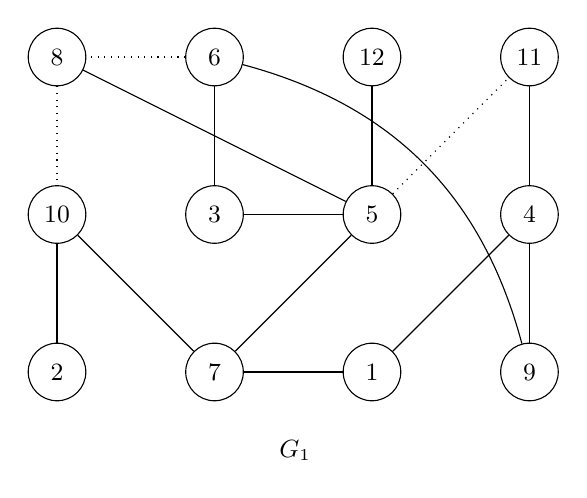
\begin{tikzpicture}
		\tikzset{text width={width("10")},
			align=center,
			font=\small}
		\tikzset{vertex/.style = {shape=circle,draw,minimum size=1.5em}}
		\tikzset{edge/.style = {-,> = latex'}}
		% vertices
		\node[vertex] (a) at  (0,0) {2};
		\node[vertex] (b) at  (2,0) {7};
		\node[vertex] (c) at  (4,0) {1};
		\node[vertex] (d) at  (6,0) {9};
		\node[vertex] (e) at  (0,2) {10};
		\node[vertex] (f) at  (2,2) {3};
		\node[vertex] (g) at  (4,2) {5};
		\node[vertex] (h) at  (6,2) {4};
		\node[vertex] (i) at  (0,4) {8};
		\node[vertex] (j) at  (2,4) {6};
		\node[vertex] (k) at  (4,4) {12};
		\node[vertex] (l) at  (6,4) {11};

		\node (n) at  (3,-1) {$G_1$};
		
		%edges
		\draw[dotted] (j) to (i);
		\draw[edge] (j) to (f);
		\draw[edge] (e) to (a);
		\draw[dotted] (i) to (e);
		
		\draw[edge] (e) to (b);
		\draw[edge] (c) to (b);
		\draw[edge] (c) to (h);
		\draw[edge] (h) to (d);
		
		\draw[edge] (g) to (f);
		\draw[edge] (g) to (k);
		\draw[dotted] (g) to (l);
		\draw[edge] (i) to (g);
		\draw[edge][bend left] (j) to (d);
		\draw[edge] (l) to (h);
		\draw[edge] (b) to (g);
		\end{tikzpicture}
		\end{center}

		\begin{enumerate}[label={\arabic*.}]
			\item Add 1 to the queue. Remove 1 form the queue, mark 4, 7 as visited and 
			add them to the queue. Mark 1 as finished. $\{4, 7\}$
			\item Remove 4 form the queue, mark 9, 11 as visited and add them to the queue. Mark 4 finished.
			$\{7, 9, 11\}$
			\item Remove 7 form the queue, mark 5, 10 as visited and add them to the queue. Mark 7 finished.
			$\{9, 11, 5, 10\}$
			\item Remove 9 form the queue, mark 6 as visited and add it to the queue. Mark 9 finished.
			$\{11, 5, 10, 6\}$
			\item Remove 11 form the queue. Mark 11 finished.
			$\{5, 10, 6\}$
			\item Remove 5 form the queue, mark 3, 8, 12 as visited and add them to the queue. Mark 5 finished.
			$\{10, 6, 3, 8, 12\}$
			\item Remove 10 form the queue, mark 2 as visited and add it to the queue. Mark 10 finished.
			$\{6, 3, 8, 12, 2\}$
			\item Remove 6 form the queue. Mark 6 finished.
			$\{3, 8, 12, 2\}$
			\item Remove 3 form the queue. Mark 3 finished. $\{8, 12, 2\}$
			\item Remove 8 form the queue. Mark 8 finished. $\{12, 2\}$
			\item Remove 12 form the queue. Mark 12 finished. $\{2\}$
			\item Remove 2 form the queue. Mark 2 finished. $\{\}$
		\end{enumerate}
	\Q{2} Is $G_1$ bipartite? Justify your answer with reference to the BFS tree.
	
		No. Since we can bipartite a tree by putting vertices in odd levels into one set and even levels into 
		another, BFS tree is bipartite. But 5 and 11 are in the same level and $(5, 11) \in E(G)$. Hence G is 
		not biparitite.

	\Q{2} Repeat part (a) on the directed graph $G_2$.
	\begin{center}
		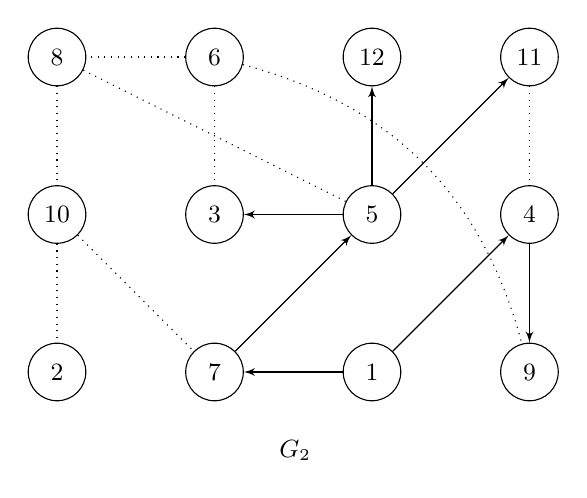
\begin{tikzpicture}
			\tikzset{text width={width("10")},
					align=center,
					font=\small}
			\tikzset{vertex/.style = {shape=circle,draw,minimum size=1.5em}}
			\tikzset{edge/.style = {->,> = latex'}}
			% vertices
			\node[vertex] (a) at  (0,0) {2};
			\node[vertex] (b) at  (2,0) {7};
			\node[vertex] (c) at  (4,0) {1};
			\node[vertex] (d) at  (6,0) {9};
			\node[vertex] (e) at  (0,2) {10};
			\node[vertex] (f) at  (2,2) {3};
			\node[vertex] (g) at  (4,2) {5};
			\node[vertex] (h) at  (6,2) {4};
			\node[vertex] (i) at  (0,4) {8};
			\node[vertex] (j) at  (2,4) {6};
			\node[vertex] (k) at  (4,4) {12};
			\node[vertex] (l) at  (6,4) {11};
			
			\node (n) at  (3,-1) {$G_2$};
			
			%edges
			\draw[dotted] (j) to (i);
			\draw[dotted] (j) to (f);
			\draw[dotted] (e) to (a);
			\draw[dotted] (i) to (e);
			
			\draw[dotted] (e) to (b);
			\draw[edge] (c) to (b);%
			\draw[edge] (c) to (h);%
			\draw[edge] (h) to (d);%
			
			\draw[edge] (g) to (f);%
			\draw[edge] (g) to (k);%
			\draw[edge] (g) to (l);%
			\draw[dotted] (i) to (g);
			\draw[dotted][bend left] (j) to (d);
			\draw[dotted] (l) to (h);
			\draw[edge] (b) to (g);%
			\end{tikzpicture}
	\end{center}
	\begin{enumerate}[label={\arabic*.}]
		\item Add 1 to the queue. Remove 1 form the queue, mark 4, 7 as visited and 
		add them to the queue. Mark 1 as finished.
		\item Remove 4 form the queue, mark 9 as visited and add it to the queue. Mark 4 finished.
		\item Remove 7 form the queue, mark 5 as visited and add it to the queue. Mark 7 finished.
		\item Remove 9 form the queue. Mark 9 finished.
		\item Remove 5 form the queue, mark 3, 11, 12 as visited and add them to the queue. Mark 5 finished.
		\item Remove 3 form the queue. Mark 3 finished.
		\item Remove 11 form the queue. Mark 11 finished.
		\item Remove 12 form the queue. Mark 12 finished.
	\end{enumerate}
	
	\newpage
	\Q{2} Run the depth-first search algorithm on the undirected graph $G_1$, starting from vertex 1, and trace the algorithm (i.e., indicate the action that is taken at every time step). When you have to choose which vertex to process next (and that choice is not otherwise specified by the DFS algorithm), use the one with the smallest label. (You do not need to draw the DFS tree.)
	\begin{center}
		\begin{enumerate}[label={\arabic*.}]
			\item Mark 1 as visited. Call DFS($G_1$, 4).
			\item Mark 4 as visited. Call DFS($G_1$, 9).
			\item Mark 9 as visited. Call DFS($G_1$, 6).
			\item Mark 6 as visited. Call DFS($G_1$, 3).
			\item Mark 3 as visited. Call DFS($G_1$, 5).
			\item Mark 5 as visited. Call DFS($G_1$, 8).
			\item Mark 8 as visited. Call DFS($G_1$, 10).
			\item Mark 10 as visited. Call DFS($G_1$, 2).
			\item Mark 2 as visited. Mark 2 as finished.
			\item Call DFS($G_1$, 7).
			\item Mark 7 as visited. Mark 7 as finished.
			\item Mark 10 as finished.
			\item Mark 8 as finished.
			\item Call DFS($G_1$, 11).
			\item Mark 11 as visited. Mark 11 as finished.
			\item Call DFS($G_1$, 12).
			\item Mark 12 as visited. Mark 12 as finished.
			\item Mark 5 as finished.
			\item Mark 3 as finished.
			\item Mark 6 as finished.
			\item Mark 9 as finished.
			\item Mark 4 as finished.
			\item Mark 1 as finished.
		\end{enumerate}
	\end{center}	

\newpage
	\Q{2} Repeat (d) on the directed graph $G_2$.
	\begin{center}
		\begin{enumerate}[label={\arabic*.}]
			\item Mark 1 as visited. Call DFS($G_1$, 4).
			\item Mark 4 as visited. Call DFS($G_1$, 9).
			\item Mark 9 as visited. Mark 9 as finished.
			\item Mark 4 as finished.
			\item Call DFS($G_1$, 7).
			\item Mark 7 as visited. Call DFS($G_1$, 5).
			\item Mark 5 as visited. Call DFS($G_1$, 3).
			\item Mark 3 as visited. Mark 3 as finished.
			\item Call DFS($G_1$, 11).
			\item Mark 11 as visited. Mark 11 as finished.
			\item Mark 12 as visited. Mark 12 as finished.
			\item Mark 5 as finished.
			\item Mark 7 as finished.
			\item Mark 1 as finished.
		\end{enumerate}
	\end{center}
	
	\Q{2} Is $G_2$ strongly connected? justify your answer with reference to a search tree (or trees).
	
	No. Since the the FDS tree does not contain all the vertices in $G_2$, there is no path form 1 to 6. Hence 
	it is not strongly connected.

\end{enumerate}

\newpage
\begin{figure}[h]
\centerline{\includegraphics[height=7cm]{scorpion.png}}
\caption{A scorpion graph}\label{scorpion}
\end{figure}

\Q{15} A scorpion graph is an undirected graph with $n$ nodes, where one node
(the body) has degree $n-2$, and is connected to $n-3$ nodes (each called a feet) and to the tail.
The tail has degree $2$, and connects to sting, which has degree $1$. A
feet is not connected to either tail or sting, and may or may not be connected to other feet.
See Figure~\ref{scorpion}. For parts (a)-(c) below, assume were given an undirected graph $G$ in an {\em adjacency matrix} representation (*not* an adjacency list).
  
\begin{enumerate}

\Q{3} Suppose we are given an undirected graph $G$ and node $s$ as a candidate sting. Give an O(n)-time procedure that returns the following: return YES if $s$ is indeed a sting and $G$ is a scorpion graph; return NO otherwise.

Let $degree(v)$ reuturns the number of 1's in $G[v]$ for some $v \in V(G)$.

\begin{algorithm}[h]
	\caption{IsScorpionSting($G, s$)}
	\If{$n < 3$} {
		\Return{NO}
	}
	\If{$degree(s) \neq 1$}{
		\Return{NO}
	}
	Let $tail$ be $s$'s only neighbour\\
	\If{$degree(tail) \neq 2$}{
		\Return{NO}
	}
	Let $body$ be $tail$'s neighbour that is not $s$\\
	\If{$degree(body) \neq n - 2$} {
		\Return{NO}
	}
	\Return{YES}
\end{algorithm}

\textbf{Proof of Correctness:} We first check whether $degree(s) = 1$. If not $G$ is not scorpion. Otherwise, 
we check if $degree(tail) = 2$. If not just return NO. Since we choose $tail$ from $s$'s neighbour set and 
$G$ is undirected. Hence $(tail,s) \in E(G)$. We then take the other neighbour of $tail$ that is not $s$. 
We already know that $body$ is not a neighbour of $string$ since $s$'s only neighbour is $tail$. We also 
know that $(body, tail) \in E(G)$. We have checked the degree of $tail$ and $sting$, so for all $feet$, 
$(feet, tail) \in E(G)$ and $(feet, sting) \in E(G)$. Thus we only need to check if 
$degree(body) = n - 2 = \lvert V(G) \rvert - 2$.

\textbf{Runtime Analysis:} Since $degree()$ takes $O(n)$ time, $T(n) = 3 O(n) + O(1) = O(n)$

\Q{2} Suppose we are given an undirected graph $G$ and a node $b$ as a candidate body. Give an O(n)-time procedure that returns the following: return YES if $b$ is indeed a body and $G$ is a scorpion graph; return NO otherwise.

\begin{algorithm}[h]
	\caption{IsScorpionBody($G, b$)}
	\If{$degree(b) \neq n - 2$} {
		\Return{NO}
	}
	Let $sting$ be a vertex that is not neighbour of $b$\\
	\If{$degree(sting) \neq 1$}{
		\Return{NO}
	}
	Let $tail$ be $sting$'s only neighbour\\
	\If{$degree(tail) \neq 2$}{
		\Return{NO}
	}
	\Return{YES}
\end{algorithm}

\textbf{Proof of Correctness:} If the number of neighbours of $b$ is not $n - 2$. Then $b$ is not a body.
If $G$ is a scorpion, the only vertex that is not neighbour of $b$ should be $sting$. 
We then check if the candidate of $sting$ is actually 
a $sting$ by calculating the degree of the candidate. Lastly, we check the candidate of $tail$.

\textbf{Runtime Analysis:} Since $degree()$ takes $O(n)$ time, $T(n) = 3 O(n) + O(1) = O(n)$.

\newpage
\Q{10} Design an O(n)-time algorithm that decides if $G$ is a scorpion graph or not. [Hint: Think about how you can identify a single sting or body node in O(n) time.].

\begin{algorithm}[h]
	\caption{IsScorpion($G$)}
	randomly pick a vertex $v$\\
	$d = degree(v)$\\
	\uIf{$d = n - 2$}{
		\Return{IsScorpionBody($G, v$)}
	} \uElseIf{$d = 1$}{
		\Return{IsScorpionSting($G, v$)}
	} \uElseIf{$d = 2$} {
		Let $u_1$ and $u_2$ be the neighbours of $v$\\
		\Return{IsScorpionBody($G, u_1$) \textbf{or} IsScorpionBody($G, u_2$)}
	} \Else{
		Let $Nbr$ be the set of neighbours of $v$\\
		$NonNbr = V(G) \backslash Nbr$\\
		$i = 0; j = 0$\\
		\While{$i < |Nbr|$ \textbf{and} $j < |NonNbr|$} {
			\uIf{$G[Nbr[i]][NonNbr[j]] = 1$}{
				$j = j + 1$\\
			} \Else{
				$i = i + 1$\\
			}
		}
		\uIf{$j < |NonNbr|$}{
			\Return{IsScorpionSting($G, NonNbr[j]$)}
		}
		\Return{NO}
	}
\end{algorithm}

\textbf{Proof of Correctness:} If $degree(v) = n - 2, 1$, then we know $v$ is a candidate for being a body or 
sting respectively. We can just using the algorithm in part (a) or (b) to check if $G$ is a scorpion. If 
$degree(v) = 2$, $v$ is a foot or tail. Either a foot or tail is neighbour of body, we can call the algorithm 
in part (b) to check if $G$ is a scorpion.\\
If $v$ is a foot with $degree(v) \geq 2$. If there exists a vertex $u$ in the set $NonNbr = V(G) \backslash Nbr$ 
that is not adjacent to any vertices in $Nbr$, $u$ is a candidate for being a sting.If a vertex is a foot or 
tail form $NonNbr$, then at some iteration, $G[Nbr[i]][NonNbr[j]] = 1$. Since a foot or tail is adjacent to 
body which is in $Nbr$. Meanwhile, we increment $i$ or $j$ at each iteration, so the loop will always 
terminates. Hence we only need to check if $NonNbr[j]$ is a sting and $G$ is a scorpion.

\textbf{Runtime Analysis:} By part (a) and (b) $IsScorpionBody()$ and $IsScorpionSting()$ takes $O(n)$ time. 
And $|Nbr| + |NonNbr| = n$, so while loop takes $O(n)$ time. $T(n) = 5 O(n) = O(n)$
\end{enumerate}



\newpage
\Q{15} Let $G=(V, E)$ be a graph with $n$ vertices and positive edge weights $c_e > 0$ on the edges, where the weights on the edges are distinct. 
Let $T=(V, E')$ be a spanning tree of $G$. Let $e_h \in T$ be the edge with the maximum edge weight. We call $e_h$ the heaviest edge of $T$. Let a spanning tree of $G$ with the minimum heaviest edge be called the minimum heaviest-edge spanning tree (MHEST). 

\begin{enumerate}
\Q{10} Prove that the MST of $G$ is also an MHEST of $G$.

Assume for a contradiction that there exists a graph $G$ where the $MST$ of $G$ is not an $MHEST$ of $G$. Let 
edge $(x, y) \in V(MST)$ where $w((x, y))$ is maximum. 
Clearly, $(x, y) \notin V(MHEST)$. There is another path $p$ from $x$ to $y$ in $MHEST$. There exists an edge 
$e$ on $p$ in MHEST such that $e \notin E(MST)$, otherwise, there is a cycle in $MST$. Since $w((x, y))$ is 
greater than all edge weights in MHEST by assumption. Let $T = E(MST) - (x, y) + e$, $w(T) < w(MST)$ 
contradicting the definition of $MST$. Hence the MST of $G$ is also an MHEST of $G$.

\Q{5}  Give a counterexample to the claim that an MHEST is always an MST.
\begin{center}
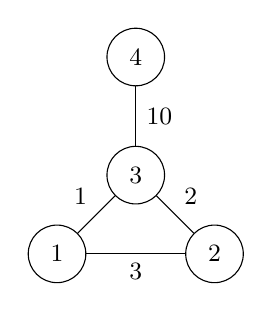
\begin{tikzpicture}
	\tikzset{text width={width("10")},
			align=center,
			font=\small}
	\tikzset{vertex/.style = {shape=circle,draw,minimum size=1em}}
	\tikzset{edge/.style = {-,> = latex'}}
	% vertices
	\node[vertex] (a) at  (0,0) {1};
	\node[vertex] (b) at  (2,0) {2};
	\node[vertex] (c) at  (1,1) {3};
	\node[vertex] (d) at  (1,2.5) {4};
	%edges
	\draw[edge] (a) to node[above, xshift = -2mm] {1} (c);
	\draw[edge] (a) to node[below] {3} (b);
	\draw[edge] (b) to node[above, xshift = 2mm] {2} (c);
	\draw[edge] (d) to node[right] {10} (c);
\end{tikzpicture}
\end{center}
Let $E(MST) = \{(1, 3), (2, 3), (3, 4)\}$, $E(MHEST) = \{(1, 3), (1, 2), (3, 4)\}$. \\
$w(MST) = 1 + 2 + 10 = 13$, but, $w(MHEST) = 1 + 3 + 10 = 14 < w(MST)$.
\end{enumerate}



\end{enumerate}

\end{document}

